\documentclass[tikz,border=15pt]{standalone}
\usetikzlibrary{positioning, arrows.meta, shapes.geometric}

\usepackage{amsmath, amssymb}

\begin{document}
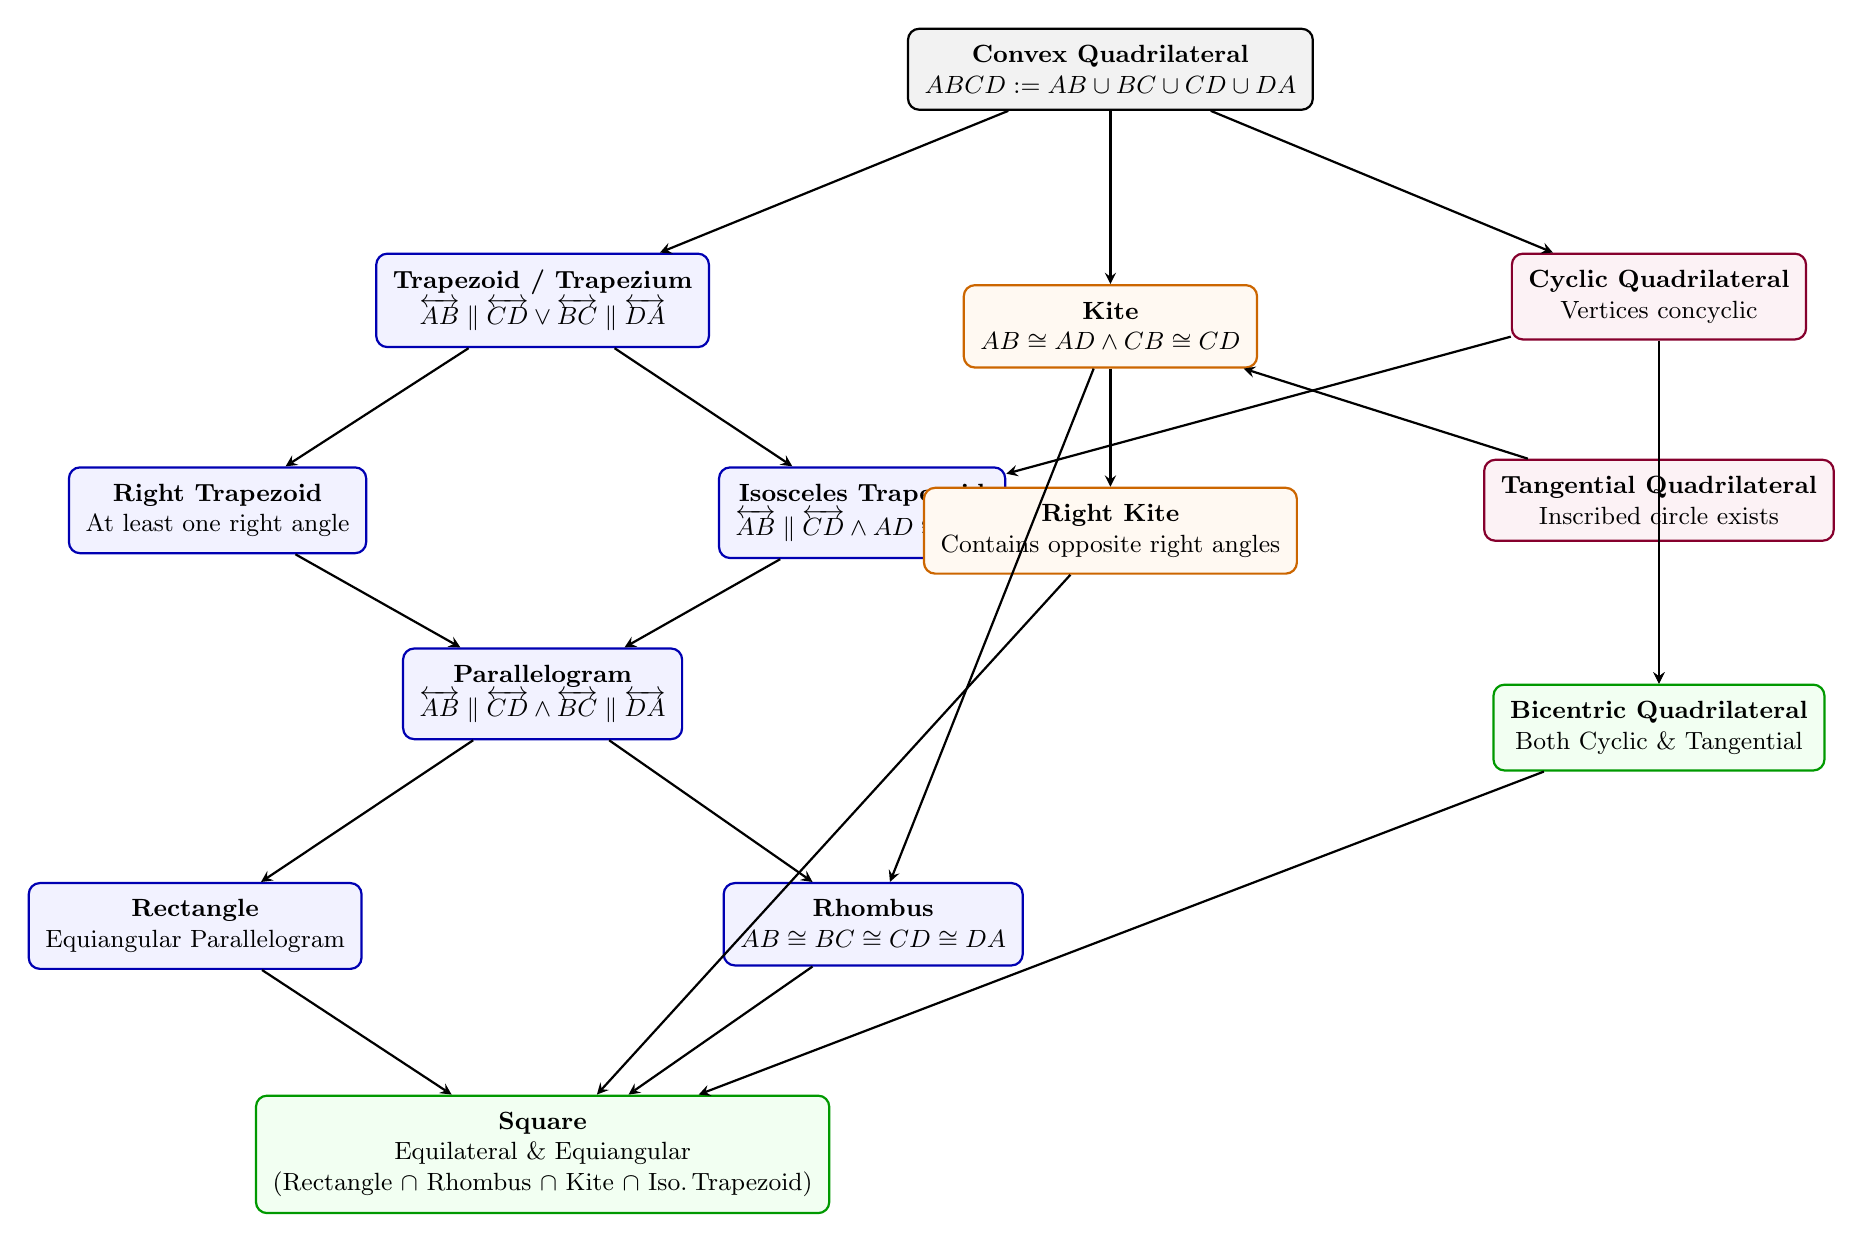
\begin{tikzpicture}[
    >=stealth,
    node distance=1.5cm and 0.4cm,
    thick,
    % Styles for different classes of geometric objects
    base/.style={rectangle, draw=black, fill=gray!10, rounded corners, inner sep=6pt, font=\small\bfseries, align=center},
    parallel/.style={rectangle, draw=blue!70!black, fill=blue!5, rounded corners, inner sep=6pt, font=\small\bfseries, align=center},
    kite/.style={rectangle, draw=orange!80!black, fill=orange!5, rounded corners, inner sep=6pt, font=\small\bfseries, align=center},
    cyclic/.style={rectangle, draw=purple!70!black, fill=purple!5, rounded corners, inner sep=6pt, font=\small\bfseries, align=center},
    hybrid/.style={rectangle, draw=green!60!black, fill=green!5, rounded corners, inner sep=6pt, font=\small\bfseries, align=center}
]

  % --- LEVEL 0: ROOT ---
  \node[base] (quad) {Convex Quadrilateral \\ \normalfont\small $ABCD := AB \cup BC \cup CD \cup DA$};

  % --- LEVEL 1: PRIMARY PARITIONS ---
  \node[parallel, below left=1.8cm and 2.5cm of quad] (trapezoid) {Trapezoid / Trapezium \\ \normalfont\small $\overleftrightarrow{AB} \parallel \overleftrightarrow{CD} \lor \overleftrightarrow{BC} \parallel \overleftrightarrow{DA}$};
  \node[kite, below=2.2cm of quad] (kite) {Kite \\ \normalfont\small $AB \cong AD \land CB \cong CD$};
  \node[cyclic, below right=1.8cm and 2.5cm of quad] (cyclic) {Cyclic Quadrilateral \\ \normalfont\small Vertices concyclic};

  % --- LEVEL 2: SECONDARY DERIVATIONS ---
  \node[parallel, below left=1.5cm and 0.1cm of trapezoid] (rtrap) {Right Trapezoid \\ \normalfont\small At least one right angle};
  \node[parallel, below right=1.5cm and 0.1cm of trapezoid] (isotrap) {Isosceles Trapezoid \\ \normalfont\small $\overleftrightarrow{AB} \parallel \overleftrightarrow{CD} \land AD \cong BC$};

  \node[parallel, below=3.8cm of trapezoid] (parallelogram) {Parallelogram \\ \normalfont\small $\overleftrightarrow{AB} \parallel \overleftrightarrow{CD} \land \overleftrightarrow{BC} \parallel \overleftrightarrow{DA}$};

  \node[kite, below=1.5cm of kite] (rkite) {Right Kite \\ \normalfont\small Contains opposite right angles};
  \node[cyclic, below=1.5cm of cyclic] (tangential) {Tangential Quadrilateral \\ \normalfont\small Inscribed circle exists};

  % --- LEVEL 3: SPECIAL PARALLELOGRAMS & HYBRIDS ---
  \node[parallel, below left=1.8cm and 0.5cm of parallelogram] (rectangle) {Rectangle \\ \normalfont\small Equiangular Parallelogram};
  \node[parallel, below right=1.8cm and 0.5cm of parallelogram] (rhombus) {Rhombus \\ \normalfont\small $AB \cong BC \cong CD \cong DA$};

  \node[hybrid, below=1.8cm of tangential] (bicentric) {Bicentric Quadrilateral \\ \normalfont\small Both Cyclic \& Tangential};

  % --- LEVEL 4: THE ULTIMATE CONVERGENCE ---
  \node[hybrid, below=4.5cm of parallelogram] (square) {Square \\ \normalfont\small Equilateral \& Equiangular \\ \normalfont\small (Rectangle $\cap$ Rhombus $\cap$ Kite $\cap$ Iso.\,Trapezoid)};

  % --- EDGES / INCLUSION LINES ---
  % Root inclusions
  \draw[->] (quad) -- (trapezoid);
  \draw[->] (quad) -- (kite);
  \draw[->] (quad) -- (cyclic);

  % Trapezoid sub-hierarchy
  \draw[->] (trapezoid) -- (rtrap);
  \draw[->] (trapezoid) -- (isotrap);
  \draw[->] (rtrap) -- (parallelogram);
  \draw[->] (isotrap) -- (parallelogram);

  % Kite sub-hierarchy
  \draw[->] (kite) -- (rkite);
  \draw[->] (kite) -- (rhombus);

  % Cyclic / Tangential sub-hierarchy
  \draw[->] (cyclic) -- (isotrap); % Isosceles trapezoids are always cyclic
  \draw[->] (cyclic) -- (bicentric);
  \draw[->] (tangential) -- (bicentric);
  \draw[->] (tangential) -- (kite); % Kites are inherently tangential

  % Parallelogram branches
  \draw[->] (parallelogram) -- (rectangle);
  \draw[->] (parallelogram) -- (rhombus);

  % Convergence to Square
  \draw[->] (rectangle) -- (square);
  \draw[->] (rhombus) -- (square);
  \draw[->] (rkite) -- (square);
  \draw[->] (bicentric) -- (square);

\end{tikzpicture}
\end{document}
